% =========================================================================== %
% Preamble                                                                    %
% =========================================================================== %

\documentclass[12pt, dvipsnames, aspectratio=169]{beamer}
%\documentclass[12pt, dipsnames, notes=only]{beamer}

\usepackage[utf8]{inputenc}
\usepackage{beamerthemesimple}

\date{November 5, 2020}
\title{bpfbox: Simple Precise Process Confinement with eBPF}
\author{\textbf{William Findlay} \and Anil Somayaji \and David Barrera}
\institute{Carleton University\\\href{mailto:will@ccsl.carleton.ca}{\ttfamily will@ccsl.carleton.ca}}

\usepackage{csquotes}
\usepackage{booktabs}

% Center floats by default
\makeatletter
\g@addto@macro\@floatboxreset{\centering}
\makeatother

\usepackage{listings}

\definecolor{listing-background}{HTML}{F7F7F7}
\definecolor{listing-rule}{HTML}{B3B2B3}
\definecolor{listing-numbers}{HTML}{B3B2B3}
\definecolor{listing-text-color}{HTML}{000000}
\definecolor{listing-keyword}{HTML}{435489}
\definecolor{listing-keyword-2}{HTML}{1284CA} % additional keywords
\definecolor{listing-keyword-3}{HTML}{9137CB} % additional keywords
\definecolor{listing-identifier}{HTML}{435489}
\definecolor{listing-string}{HTML}{00999A}
\definecolor{listing-comment}{HTML}{8E8E8E}

% Set default listings style
\lstdefinestyle{listingstyle}{
    %backgroundcolor  = \color{listing-background},
    %xleftmargin      = 2em,
    %numberstyle      = \color{listing-numbers}\ttfamily\normalsize\lst@ifdisplaystyle\scriptsize\fi,
    basicstyle       = \ttfamily\normalsize\lst@ifdisplaystyle\scriptsize\fi,
    keywordstyle     = {\color{listing-keyword}\bfseries},
    keywordstyle     = {[2]\color{listing-keyword-2}\bfseries},
    keywordstyle     = {[3]\color{listing-keyword-3}\bfseries\itshape},
    sensitive        = true,
    commentstyle     = \color{listing-comment},
    stringstyle      = \color{listing-string},
    showstringspaces = false,
    literate = {~}{$\sim$}{1}
}
\lstset{style=listingstyle}

\definecolor[named]{ACMBlue}{cmyk}{1,0.1,0,0.1}
\definecolor[named]{ACMYellow}{cmyk}{0,0.16,1,0}
\definecolor[named]{ACMOrange}{cmyk}{0,0.42,1,0.01}
\definecolor[named]{ACMRed}{cmyk}{0,0.90,0.86,0}
\definecolor[named]{ACMLightBlue}{cmyk}{0.49,0.01,0,0}
\definecolor[named]{ACMGreen}{cmyk}{0.20,0,1,0.19}
\definecolor[named]{ACMPurple}{cmyk}{0.55,1,0,0.15}
\definecolor[named]{ACMDarkBlue}{cmyk}{1,0.58,0,0.21}

\setbeamertemplate{section in toc}[sections numbered]

\hypersetup{
    colorlinks = true,
    linkcolor  = .,
    urlcolor   = ACMBlue,
    citecolor  = ACMPurple,
}
\urlstyle{tt}

\usepackage{bpfbox}

% Table of Contents for sections
\AtBeginSection[]
{
    \begin{frame}[c, noframenumbering, plain]
        \begin{center}
        \fontsize{42.99}{51.59} \selectfont \bfseries \color{destacado} \insertsection
        \end{center}
    \end{frame}
}

% =========================================================================== %
% Document                                                                    %
% =========================================================================== %

\begin{document}

\setwatermark{
\includegraphics[height=0.8\textheight]{figs/bpfbox-logo.pdf}}

% Slide Ideas:
% 1) What we did before eBPF (how eBPF unifies observability in Linux)
% 2) eBPF timeline (BTF, KRSI, etc)
% 3) a branching diagram showcasing eBPF features and security use cases
% 4) a slide with pictures of the security conversation from eBPF.io
% 5) a slide showing LSM vs eBPF LSM
% 6) Future directions for bpfbox
%      - add policy generation
%      - update policy language (yaml, rego?)
%      - implement network address filtering?
%      - new inode local storage and task local storage map types (garbage
%        collected storage for security attributes/policy in an eBPF map)
% 7) Future directions for eBPF in security

% Title page
\begin{frame}[noframenumbering, plain]
\titlepage
\vfill
\vspace{4em}
{\footnotesize Fall 2020 CCSL/CISL Talk}
\end{frame}

\setwatermark[hoffset=6cm, voffset=0.3cm]{}

\begin{frame}[c, noframenumbering, plain]{Outline of this Talk}
    \tableofcontents
\end{frame}

\section{The Process Confinement Problem}

\begin{frame}[c]{What is Process Confinement?}
We want to be able to \textbf{confine} our \textbf{processes}.
\begin{itemize}
    \item Also known as \textit{sandboxing}
\end{itemize}
\vfill
Why do we want to do this?
\begin{itemize}
    \item Default protection mechanisms are too:
    \begin{itemize}
        \item Granular
        \item User-centric
        \item Discretionary
    \end{itemize}
    \item Protection can be \textbf{overridden}
    \begin{itemize}
        \item Superuser (*nix)
        \item Administrator (Windows)
    \end{itemize}
\end{itemize}
\vfill
How do we protect the user from \textit{themselves} and \textit{their own processes}?
\end{frame}

\begin{frame}[c]{An Interesting Question}
\begin{center}
    \Huge
    How many processes do you think are running on your computer \textbf{right now}?
\end{center}
\vfill
\begin{itemize}
    \item Probably a lot more than you think
    \item You probably didn't start most of them yourself
    \item You might not even know what some of them are for
\end{itemize}
\end{frame}

\begin{frame}[t]{Threat Model}
\begin{columns}
    \begin{column}{0.45\textwidth}
        \textbf{Compromised Processes}
        \begin{itemize}
            \item Web servers
            \item Daemons
            \item Chat applications
            \item etc.
        \end{itemize}
        \vspace{2em}
        The Morris Worm
        \begin{itemize}
            \item Backdoor in \texttt{sendmail} daemon
            \item Buffer overflow in \texttt{fingerd}
            \item Estimated damage: \$100,000--\$10,000,000
        \end{itemize}
    \end{column}
    \begin{column}{0.55\textwidth}
        \color{black}
        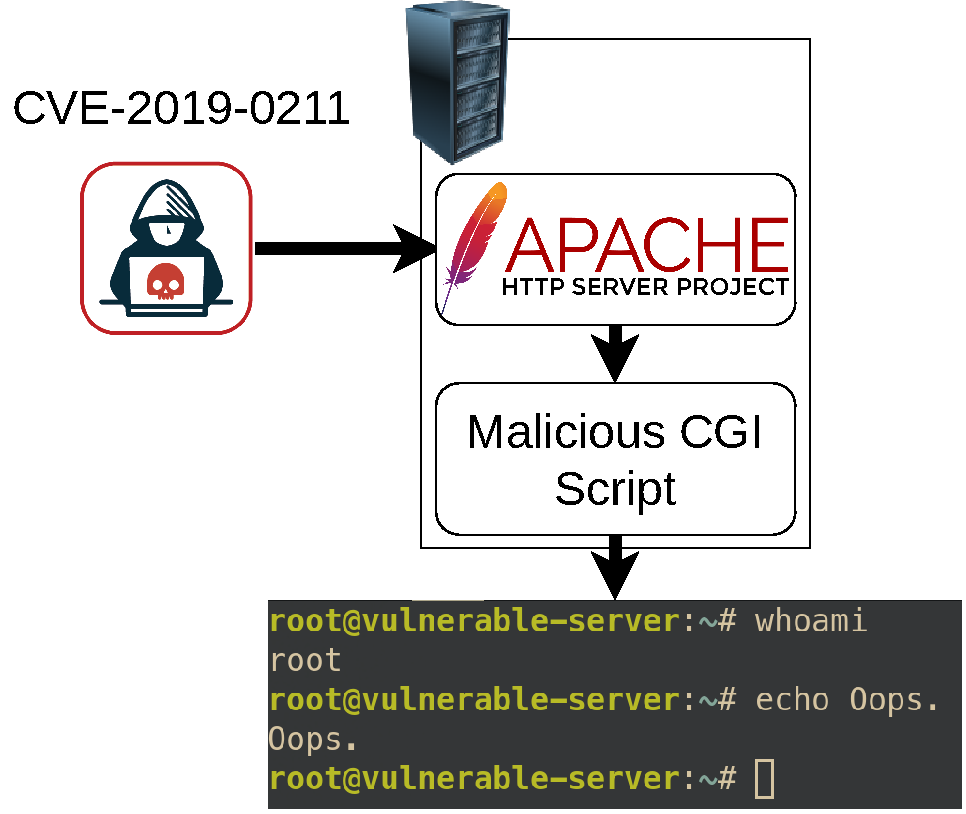
\includegraphics[width=1\textwidth]{figs/threat-model.pdf}
    \end{column}
\end{columns}
\end{frame}

\begin{frame}[t]{Threat Model}
    \textbf{Semi-Honest Software}
    \begin{itemize}
        \item Software that does its job...
        \item But also performs potentially \textbf{unwanted actions}
    \end{itemize}
    \begin{center}
        \color{black}
        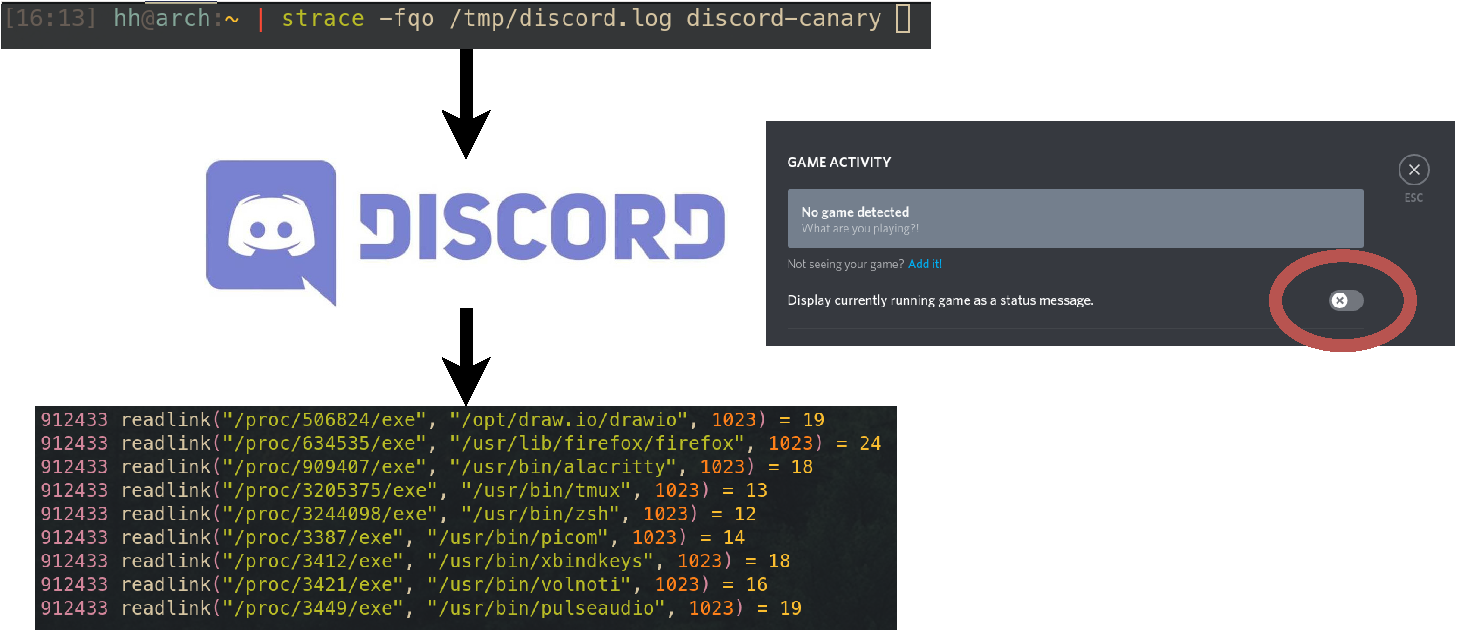
\includegraphics[width=0.7\textwidth]{figs/discord.pdf}
    \end{center}
\end{frame}

\begin{frame}[c]{Threat Model}
\begin{columns}
    \begin{column}{0.3\textwidth}
        \textbf{Malicious Software}
        \begin{itemize}
            \item Viruses
            \item Trojans
            \item Ransomware
            \item Spyware
            \item etc.
        \end{itemize}
    \end{column}
    \begin{column}{0.6\textwidth}
        \color{black}
        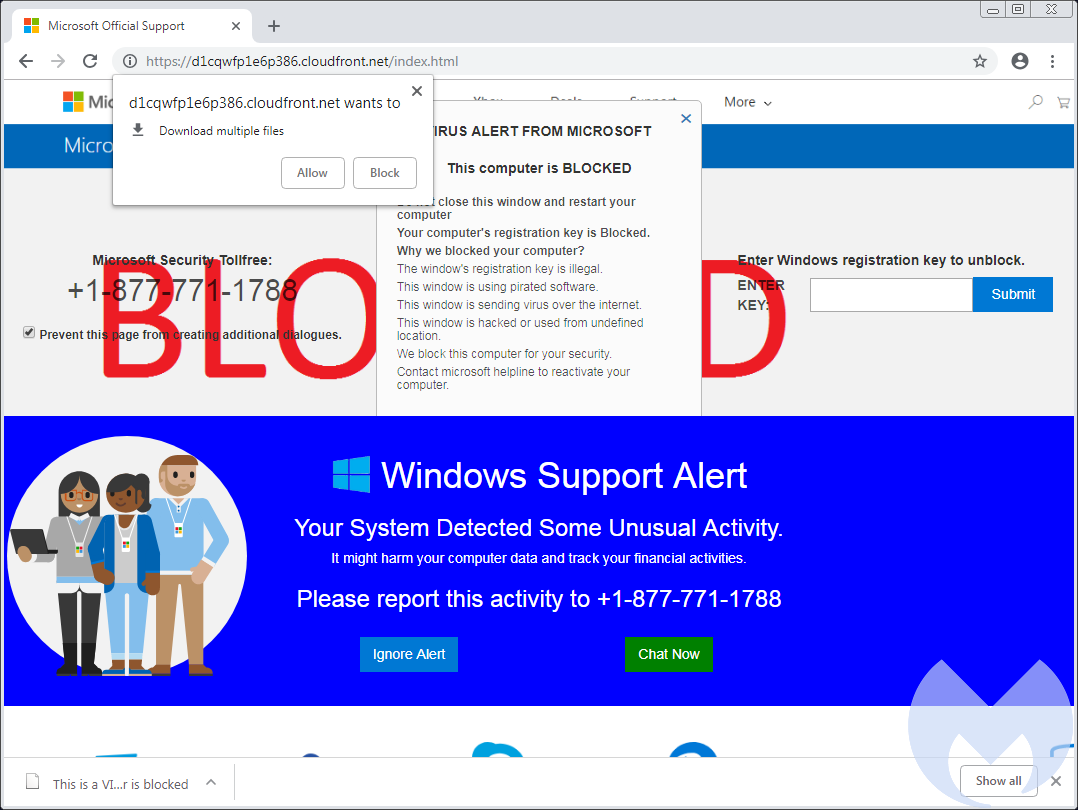
\includegraphics[width=1\textwidth]{figs/fake-av.png}
    \end{column}
\end{columns}
\end{frame}

\begin{frame}[c]{Threat Model}
\begin{columns}
    \begin{column}{0.4\textwidth}
        \textbf{Attack goals?}
        \begin{itemize}
            \item Installing backdoors/rootkits
            \item Information leakage
            \item Denial of service
            \item Data ransom
            \item Setting up a botnet
        \end{itemize}
    \end{column}
    \begin{column}{0.6\textwidth}
        \begin{center}
            \Huge
            Process confinement reduces the attack\\surface.
        \end{center}
    \end{column}
\end{columns}
\end{frame}

\begin{frame}[c]{The Process Confinement Problem}
    \begin{itemize}
        \item \enquote{A Note on the Confinement Problem} (Lampson, 1973)
        \begin{center}
            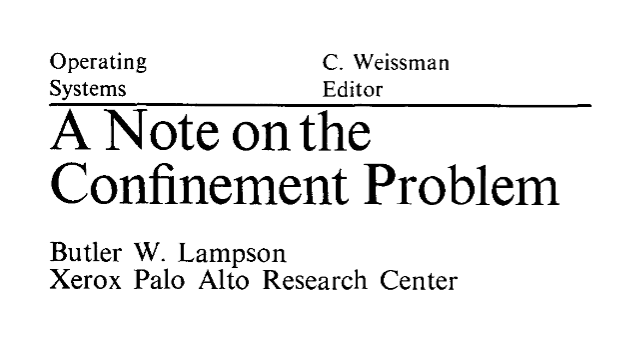
\includegraphics[width=0.6\textwidth]{figs/lampson/1.png}
        \end{center}
        \item An open problem for nearly \textbf{five decades}
    \end{itemize}
\end{frame}

%\begin{frame}[c]{But, William... We've Already Solved It...}
%    \begin{center}
%        \Huge \textbf{Have we?}
%    \end{center}
%    \vfill
%    \includegraphics{}
%\end{frame}

\section{The Status Quo}

\begin{frame}[c]{Unix DAC}

\end{frame}

\begin{frame}[c]{POSIX Capabilities}

\end{frame}

\begin{frame}[c]{Namespaces and Cgroups}

\end{frame}

\begin{frame}[c]{System Call Interposition}

\end{frame}

\begin{frame}[c]{Linux MAC}

\end{frame}

\begin{frame}[c]{Containers / Containerized Package Management}

\end{frame}

\section{eBPF 101}

\begin{frame}[c]{eBPF in the Beginning}
eBPF $\equiv$ \textbf{E}xtended \textbf{B}erkley \textbf{P}acket \textbf{F}ilter
\begin{itemize}
    \item But it has little to do with Berkley, packets, or filtering nowadays
    \item The name BPF is preserved for historical reasons
\end{itemize}
\vfill
So then \textbf{what is eBPF?}
\begin{itemize}
    \item A major re-write of the Linux BPF engine
    \begin{itemize}
        \item Alexei Starovoitov and Daniel Borkmann
    \end{itemize}
    \item Merged into the Linux kernel in 2014
    \item The original goal was fine-grained, cross-layer \textbf{system introspection}
\end{itemize}
\end{frame}

\begin{frame}[c]{What Can eBPF Do?}
\begin{center}
    \color{black}
    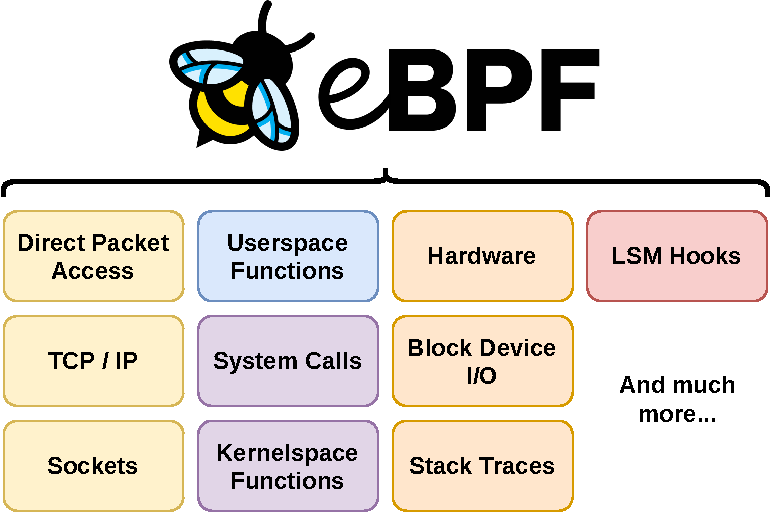
\includegraphics[height=0.8\textheight]{figs/ebpf-overview.pdf}
\end{center}
\end{frame}

\begin{frame}[c]{How eBPF Works}
\begin{center}
    \color{black}
    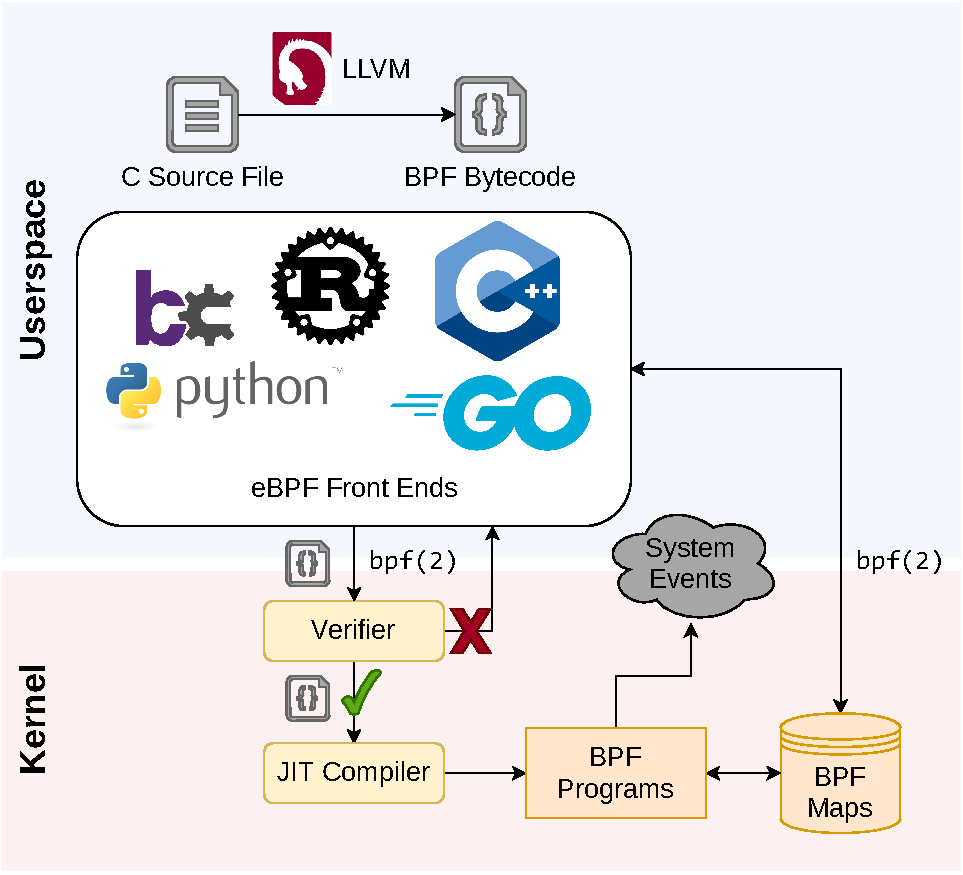
\includegraphics[height=0.8\textheight]{figs/how-ebpf-works.pdf}
\end{center}
\end{frame}

\begin{frame}[c]{Verifiably Safe Programs}
Restricted execution context.
\begin{itemize}
    \item 512 byte stack limit
    \item 11 registers (10 general purpose)
    \item Memory access must be bounds-checked
    \item No unbounded loops
    \item No back-edges in control flow
\end{itemize}
\end{frame}

\begin{frame}[c]{eBPF in 2020}
eBPF is now \textbf{more than just an observability tool}.
\begin{itemize}
    \item eBPF provides a \textbf{safe}, \textbf{efficient}, and \textbf{flexible} way for privileged users to extend the kernel
    \item eBPF turns Linux into a \textbf{programmable kernel}
\end{itemize}
\vfill
Linux 5.7 $\rightarrow$ KRSI (\textbf{K}ernel \textbf{R}untime \textbf{S}ecurity \textbf{I}nstrumentation)
\begin{itemize}
    \item Attach BPF programs to LSM hooks
    \item Make security decisions and generate audit logs with eBPF
\end{itemize}
\end{frame}

\begin{frame}[c]{KRSI: BPF LSM Programs}
\begin{itemize}
    \item TODO explain KRSI with a picture
\end{itemize}
\end{frame}

\section{bpfbox Overview}

\begin{frame}[c]{bpfbox at a Glance}
\begin{columns}
    \begin{column}{0.6\textwidth}
        \begin{itemize}
            \item bpfbox is a novel \textbf{process confinement mechanism} for Linux%
            \begin{itemize}
                \item Using a new Linux technology called eBPF
            \end{itemize}
            \vspace{2em}
            \item Users write per-application policy in a \textbf{simple policy language}
            \vspace{2em}
            \item Policy is enforced by attaching \textbf{eBPF programs} to \textbf{LSM hooks}%
            \begin{itemize}
                \item Integrates cross-layer state into policy decisions
            \end{itemize}
        \end{itemize}
    \end{column}
    \begin{column}{0.4\textwidth}
        \begin{center}
            \color{black}
            
\includegraphics[width=0.9\textwidth]{figs/bpfbox-logo.pdf}\\
        \end{center}
        \vspace{1em}
    \end{column}
\end{columns}
\end{frame}

\begin{frame}[c]{Motivation}
\begin{itemize}
    \item Existing process confinement mechanisms are \textbf{complex}
\end{itemize}
\begin{center}
    \color{black}
    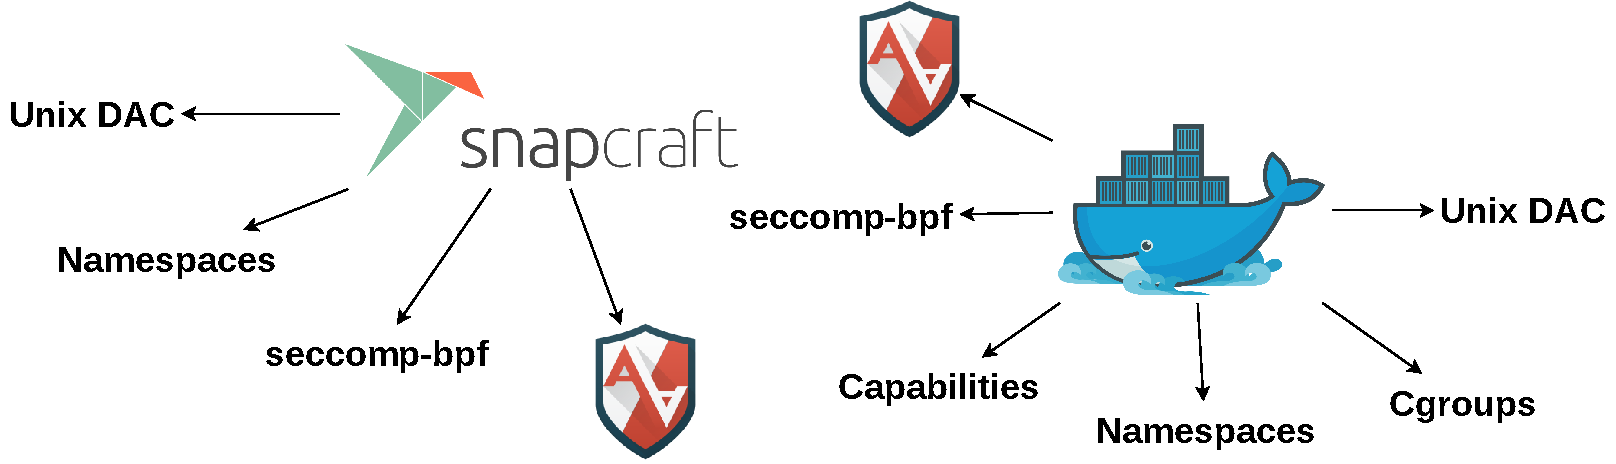
\includegraphics[width=0.8\textwidth]{figs/process-confinement-landscape.pdf}
\end{center}
\begin{itemize}
    \item Existing process confinement mechanisms are \textbf{difficult to use}
\end{itemize}
\begin{center}
    \color{black}
    
\includegraphics[height=0.2\textheight]{figs/mac.pdf}
\end{center}
\begin{itemize}
    \item Can we do any better?
\end{itemize}
\end{frame}

% TODO: do I want this? does it make sense to have it here?
%\begin{frame}[c]{Stakeholders as Policy Authors}
%\begin{itemize}
%    \item \textbf{Security experts} define the policy
%\end{itemize}
%\begin{center}
%    
\includegraphics[height=4em]{figs/selinux.png}
%    \hspace{3em}
%    
\includegraphics[height=4em]{figs/apparmor.png}
%    \hspace{3em}
%    
\includegraphics[height=4em]{figs/tomoyo.png}
%\end{center}
%
%\begin{itemize}
%    \item \textbf{Application authors} and \textbf{packagers} define the policy
%\end{itemize}
%\begin{center}
%    \includegraphics[height=4em]{figs/Snapcraft.png}
%    \hspace{3em}
%    
\includegraphics[height=4em]{figs/docker.png}
%\end{center}
%
%\begin{itemize}
%    \item \textbf{End users} define the policy
%\end{itemize}
%\begin{center}
%    \Huge ???
%\end{center}
%\end{frame}

\begin{frame}[c]{eBPF Changes the Game}
eBPF enables:
\begin{itemize}
    \item Fine-grained system introspection
    \item Integration of \textbf{cross-layer state} with policy enforcement
    \item Rapid prototyping
    \item Safe production deployment of new security solutions
\end{itemize}
\vfill
We have an opportunity to \textbf{rethink process confinement} from the ground up.
\end{frame}

% - Unix DAC, seccomp-bpf, namespaces, cgroups, Linux MAC (SELinux, AppArmor,
%   TOMOYO, etc.)
% - Where does this complexity arise from? No unified solution
% (Maybe the following can go into a separate slide...)
% - Higher level frameworks as Frankenstein's monster
% - Higher level frameworks being too coarse-grained (Snap vs bpfbox)

\section{bpfbox Design and Implementation}

\begin{frame}[c]{bpfbox Implementation}
\begin{columns}
    \begin{column}{0.66\textwidth}
        \begin{itemize}
            \item Userspace daemon using the Python3 bcc framework
            \vspace{2em}
            \item Kernelspace components are all written in eBPF
            \begin{itemize}
                \item LSM probes (KRSI), kprobes, uprobes
                \item Under 2000 source lines of kernelspace code
            \end{itemize}
            \vspace{2em}
            \item Thanks to eBPF, bpfbox is \textbf{light-weight}, \textbf{flexible}, and \textbf{production-safe}
            \begin{itemize}
                \item Works out of the box on any vanilla Linux kernel $\ge 5.8$
            \end{itemize}
        \end{itemize}
    \end{column}
    \begin{column}{0.33\textwidth}
        \begin{center}
            \color{black}
            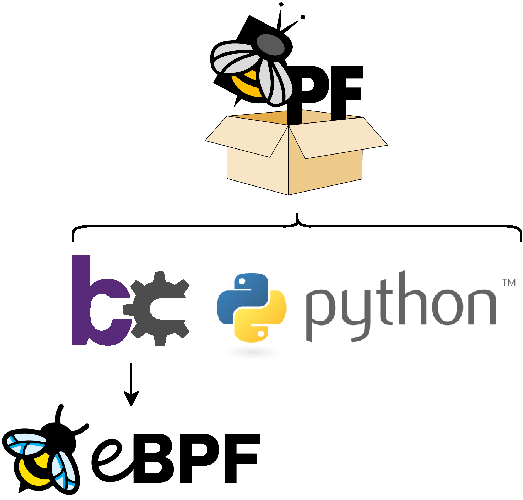
\includegraphics[width=0.9\textwidth]{figs/at-a-glance.pdf}
        \end{center}
        \vspace{2em}
    \end{column}
\end{columns}
\end{frame}

\begin{frame}[c]{bpfbox Architecture}
\begin{center}
    \color{black}
    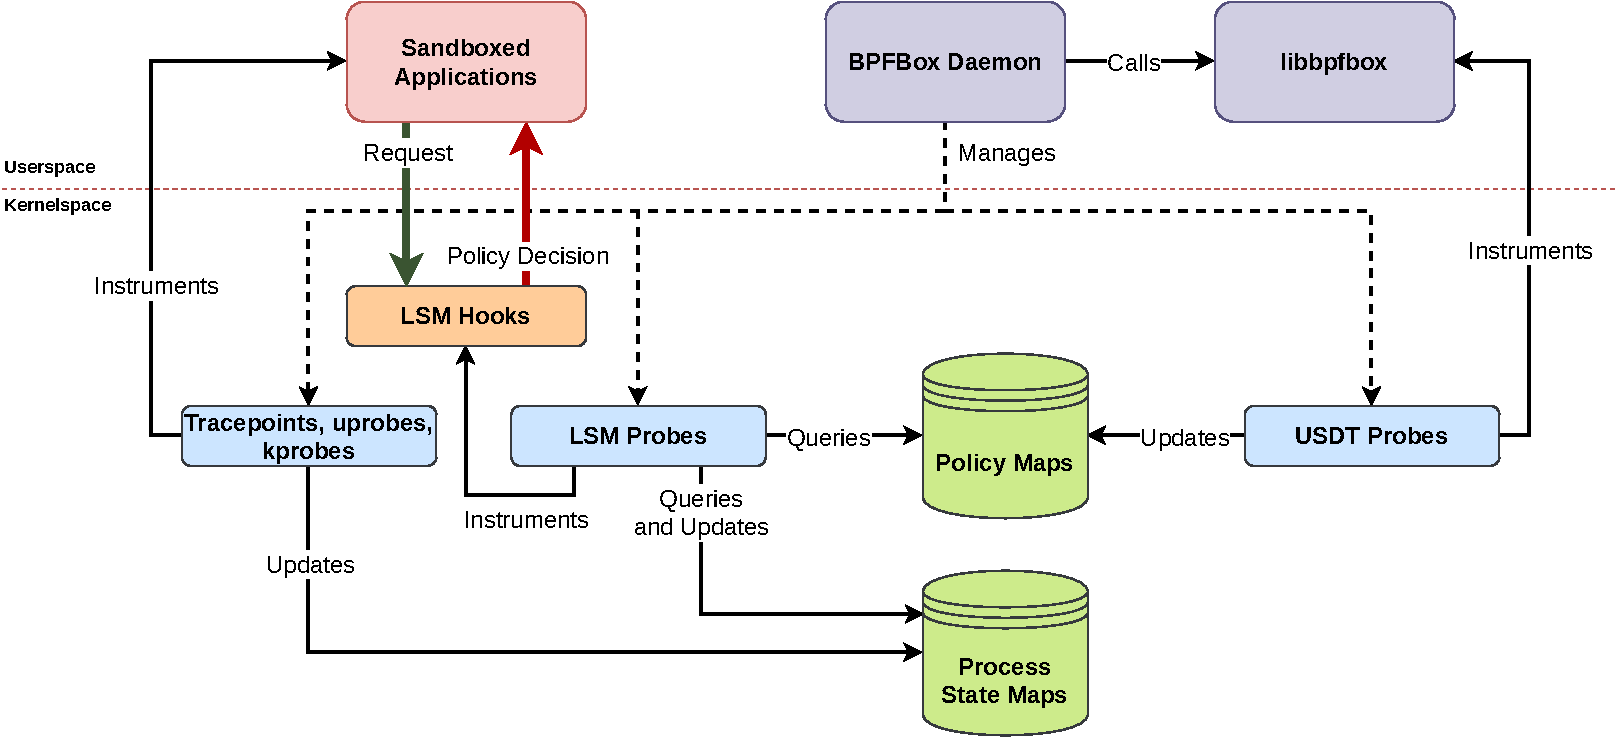
\includegraphics[width=1\textwidth]{figs/bpfbox-overview.pdf}
\end{center}
\end{frame}

%\begin{frame}[c, noframenumbering]{bpfbox Architecture}
%\begin{center}
%    \color{black}
%    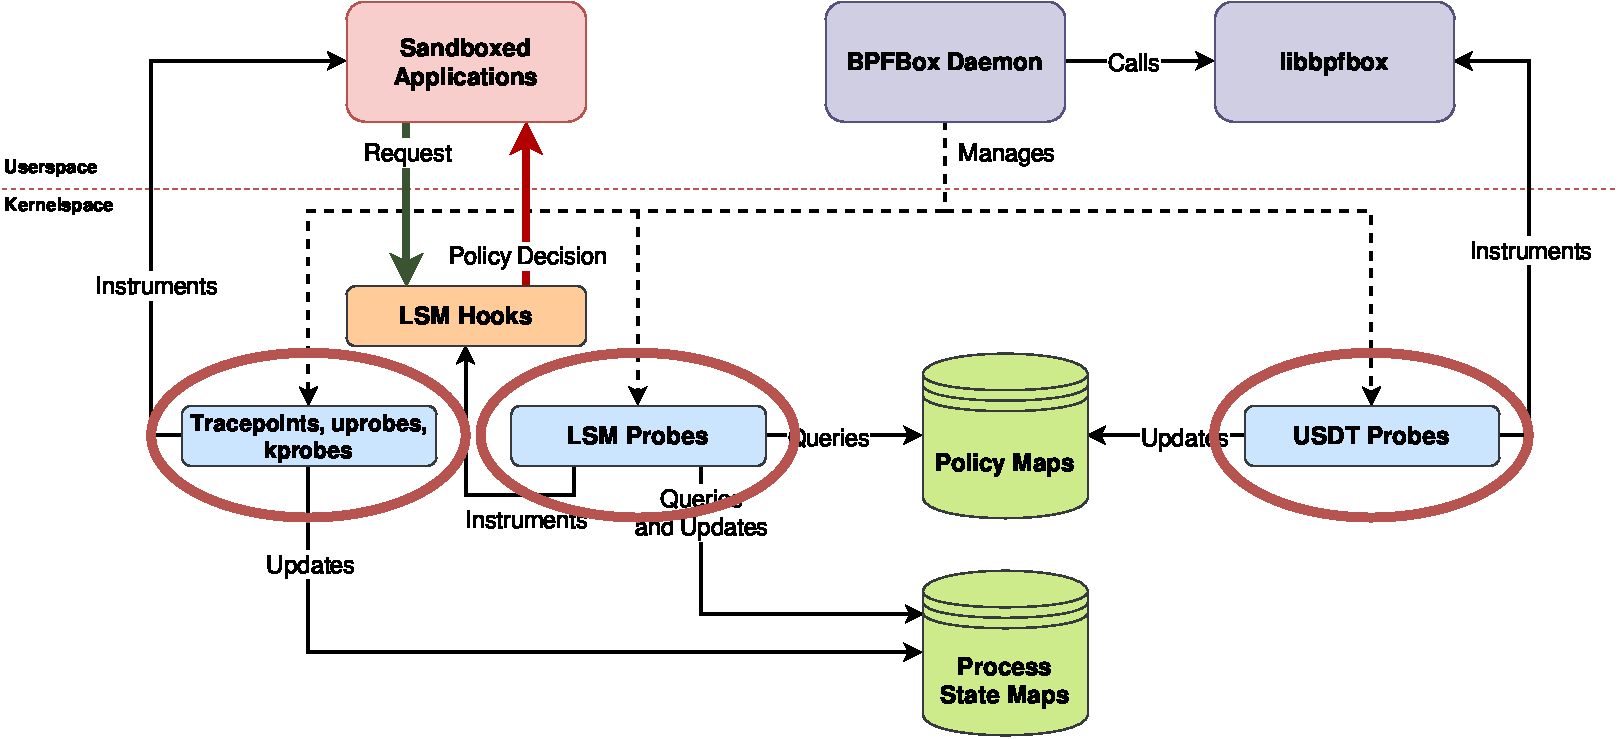
\includegraphics[width=1\textwidth]{figs/bpfbox-overview-1.pdf}
%\end{center}
%\end{frame}
%
%\begin{frame}[c, noframenumbering]{bpfbox Architecture}
%\begin{center}
%    \color{black}
%    \vspace{0.55em}
%    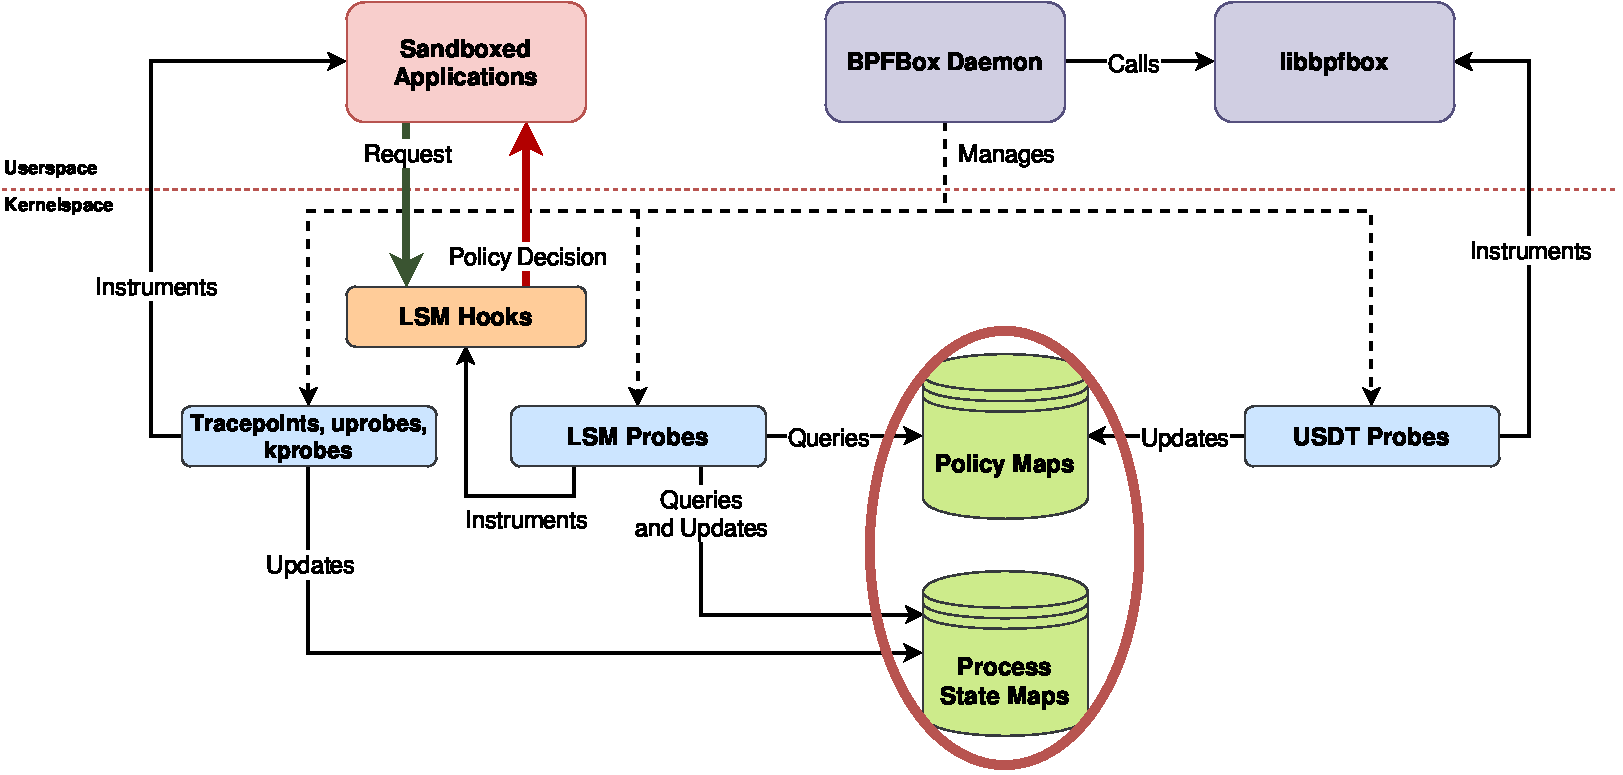
\includegraphics[width=1\textwidth]{figs/bpfbox-overview-2.pdf}
%\end{center}
%\end{frame}
%
%\begin{frame}[c, noframenumbering]{bpfbox Architecture}
%\begin{center}
%    \color{black}
%    \vspace{-0.2em}
%    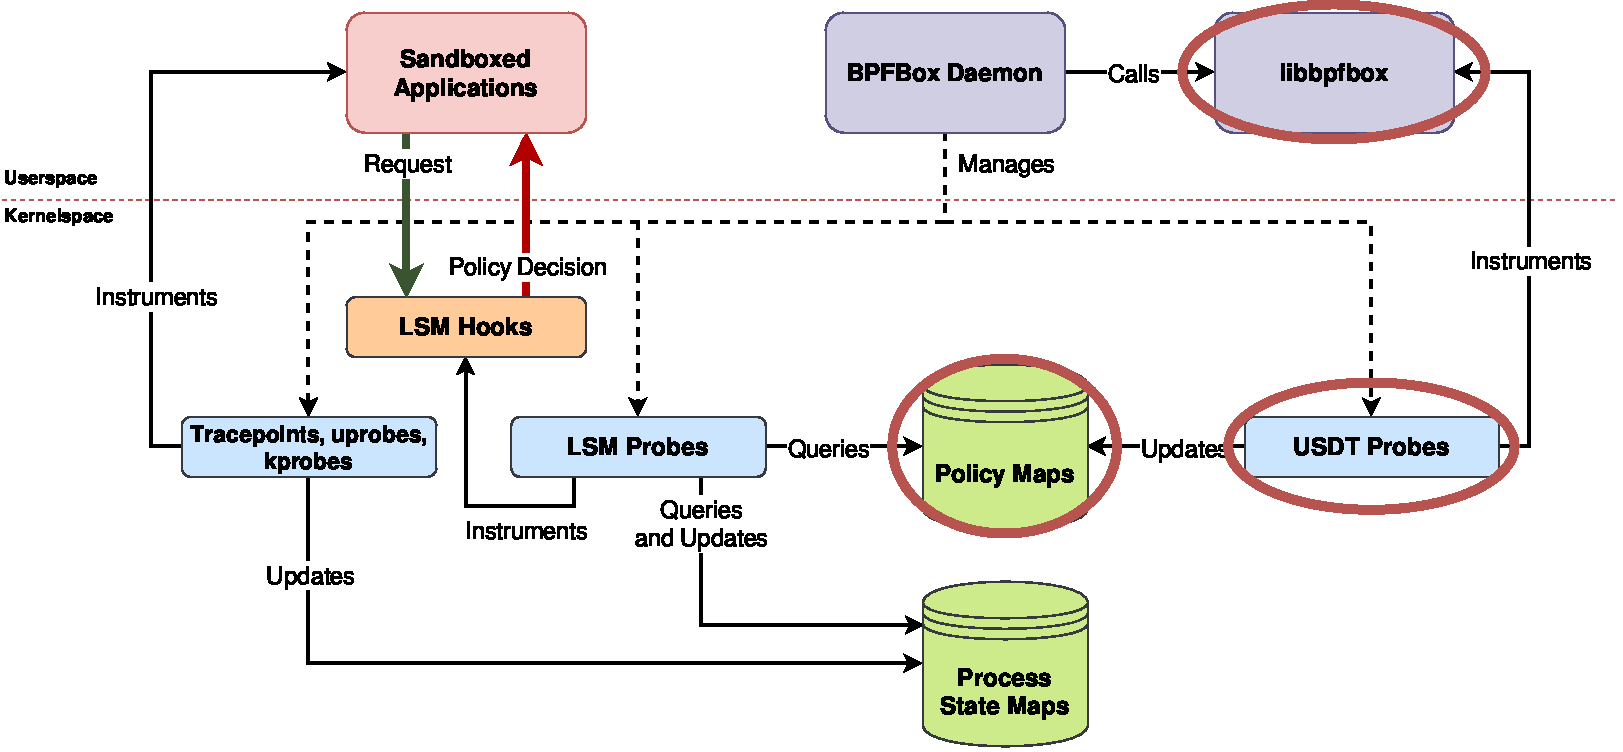
\includegraphics[width=1\textwidth]{figs/bpfbox-overview-3.pdf}
%\end{center}
%\end{frame}
%
%\begin{frame}[c, noframenumbering]{bpfbox Architecture}
%\begin{center}
%    \color{black}
%    \vspace{0.5em}
%    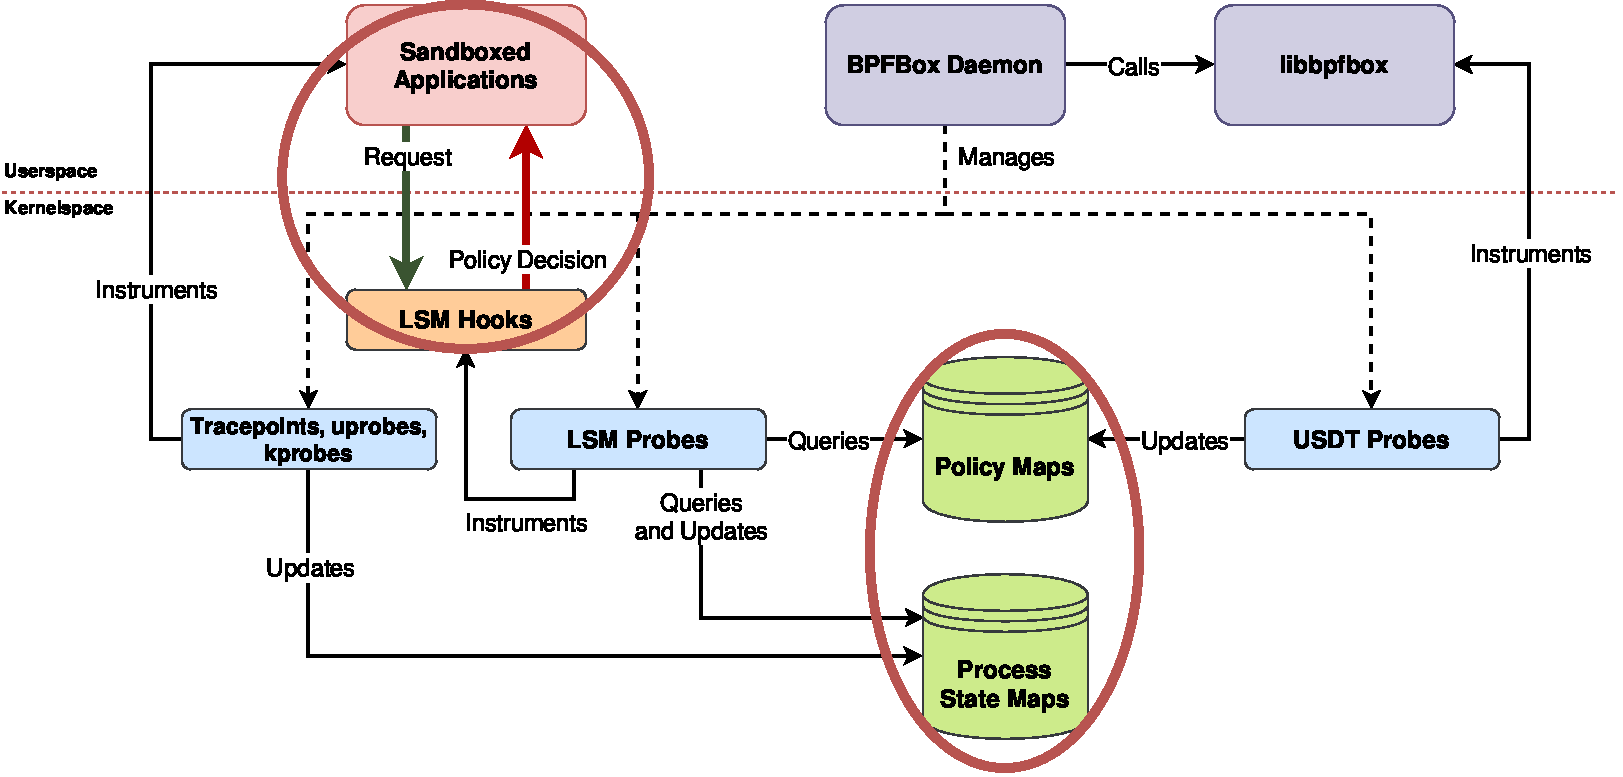
\includegraphics[width=1\textwidth]{figs/bpfbox-overview-4.pdf}
%\end{center}
%\end{frame}

\begin{frame}[c]{Policy Design Goals}
\begin{enumerate}
    \item \textbf{Simplicity}
    \begin{itemize}
        \item Policy should be simple enough for ad hoc confinement
    \end{itemize}
    \vfill
    \item \textbf{Application transparency}
    \begin{itemize}
        \item Policy should not require changes to the confined application
    \end{itemize}
    \vfill
    \item \textbf{Flexibility}
    \begin{itemize}
        \item Policy should offer optional layers of granularity
    \end{itemize}
    \vfill
    \item \textbf{Security}
    \begin{itemize}
        \item Policy should follow the principle of least privilege
        \item It should be difficult to write an insecure policy
    \end{itemize}
\end{enumerate}
\end{frame}

\begin{frame}[c, fragile]{Rules and Directives}
\textit{Rules} specify access to system objects:
\begin{itemize}
    \item \lstinline[language=bpfbox]|fs(file, access)|
    \item \lstinline[language=bpfbox]|net(socket, access)|
    \item \lstinline[language=bpfbox]|signal(prog, sig)|
    \item etc.
\end{itemize}

\vfill
\textit{Directives} augment blocks of rules:
\begin{itemize}
    \item \lstinline[language=bpfbox]|#[directive]| syntax
    \item Specify \textbf{actions to be taken} on a block of rules
    \item Add \textbf{additional context} to a block of rules
\end{itemize}
\end{frame}

\begin{frame}[c, fragile]{Taints and Transitions}
\begin{itemize}
    \item \lstinline[language=bpfbox]|#[taint]|  $\rightarrow$ Start confinement
    \item \lstinline[language=bpfbox]|#[transition]|  $\rightarrow$ Switch profiles on \texttt{execve}
\end{itemize}
\vfill
\begin{lstlisting}[language=bpfbox, xleftmargin=.25\textwidth]
#![profile "/bin/mywebdaemon"]

#[taint] {
    net(inet, any)
    net(inet6, any)
}

/* ... */

#[transition] {
    fs("/bin/myhelper", getattr|read|exec)
}
\end{lstlisting}
\end{frame}

\begin{frame}[c, fragile]{Policy at the Function Call Level}
\begin{itemize}
    \item \lstinline[language=bpfbox]|#[func "foo"]|  $\rightarrow$ Apply rules only within a call to \texttt{foo()}
    \item \lstinline[language=bpfbox]|#[kfunc "foo"]|  $\rightarrow$ Same thing, but for kernel functions
\end{itemize}
\vfill
\begin{lstlisting}[language=bpfbox, xleftmargin=.25\textwidth]
#![profile "/sbin/mylogin"]

#[func "check_password"]
#[allow] {
    fs("/etc/passwd", read)
    fs("/etc/shadow", read)
}

#[func "add_user"]
#[allow] {
    fs("/etc/passwd", read|append)
    fs("/etc/shadow", read|append)
}

/* ... */
\end{lstlisting}
\end{frame}

% TODO: add this back in?
%\begin{frame}[t]{bpfbox vs.~Snap}
%\begin{columns}
%    \begin{column}{0.5\textwidth}
%        \hfill
\includegraphics[height=3em]{figs/bpfbox-logo.pdf}\hfill
%        \begin{itemize}
%            \item
%        \end{itemize}
%    \end{column}
%
%    \begin{column}{0.5\textwidth}
%        \hfill
\includegraphics[height=3em]{figs/snapcraft.png}\hfill
%        \begin{itemize}
%            \item
%        \end{itemize}
%    \end{column}
%\end{columns}
%\vfill
%\vfill
%\vfill
%\vfill
%\vfill
%\vfill
%\vfill
%See our paper for a detailed case study of Apache \texttt{httpd} policy.
%\end{frame}

\section{bpfbox Performance Evaluation}

\begin{frame}[c]{Methodology}
\begin{itemize}
    \item Phoronix Test Suite OSBench
    \begin{itemize}
        \item Measures basic OS functionality
        \item (spawning processes, memory allocations, etc.)
    \end{itemize}

    \vfill
    \item Phoronix Test Suite Apache
    \begin{itemize}
        \item Benchmark Apache \texttt{httpd} packets per second
    \end{itemize}

    \vfill
    \item Kernel compilation benchmarks
    \begin{itemize}
        \item Measure Linux kernel compilation performance
        \item Heavy workload, spawning lots of processes
    \end{itemize}
\end{itemize}
\end{frame}

\begin{frame}[c]{Methodology}
Two modes of operation for each test.
\vfill
\begin{itemize}
    \item Passive mode
    \begin{itemize}
        \item bpfbox and AppArmor instrument hooks, but do not enforce or audit
        \item Test lowest possible overhead
    \end{itemize}
    \vfill
    \item Complaining mode
    \begin{itemize}
        \item bpfbox and AppArmor complain about (log) every security-sensitive operation
        \item Test worst case overhead
    \end{itemize}
\end{itemize}
\end{frame}

\begin{frame}[c]{Results}
\begin{itemize}
    \item Phoronix OSBench
    \begin{itemize}
        \item Passive: bpfbox is \textbf{roughly equivalent} to AppArmor
        \item Complaining: bpfbox performs \textbf{significantly better} than AppArmor
    \end{itemize}

    \vfill
    \item Phoronix Apache
    \begin{itemize}
        \item bpfbox and AppArmor are \textbf{roughly equivalent}
    \end{itemize}

    \vfill
    \item Kernel compilation
    \begin{itemize}
        \item Passive: bpfbox is \textbf{roughly equivalent} to AppArmor
        \item Complaining: bpfbox performs \textbf{better in kernelspace} overhead and \textbf{worse in userspace} overhead
    \end{itemize}
\end{itemize}
\end{frame}

\section{The Future of eBPF and Security}

\begin{frame}[c]{Security Applications of eBPF}
\begin{center}
    \color{black}
    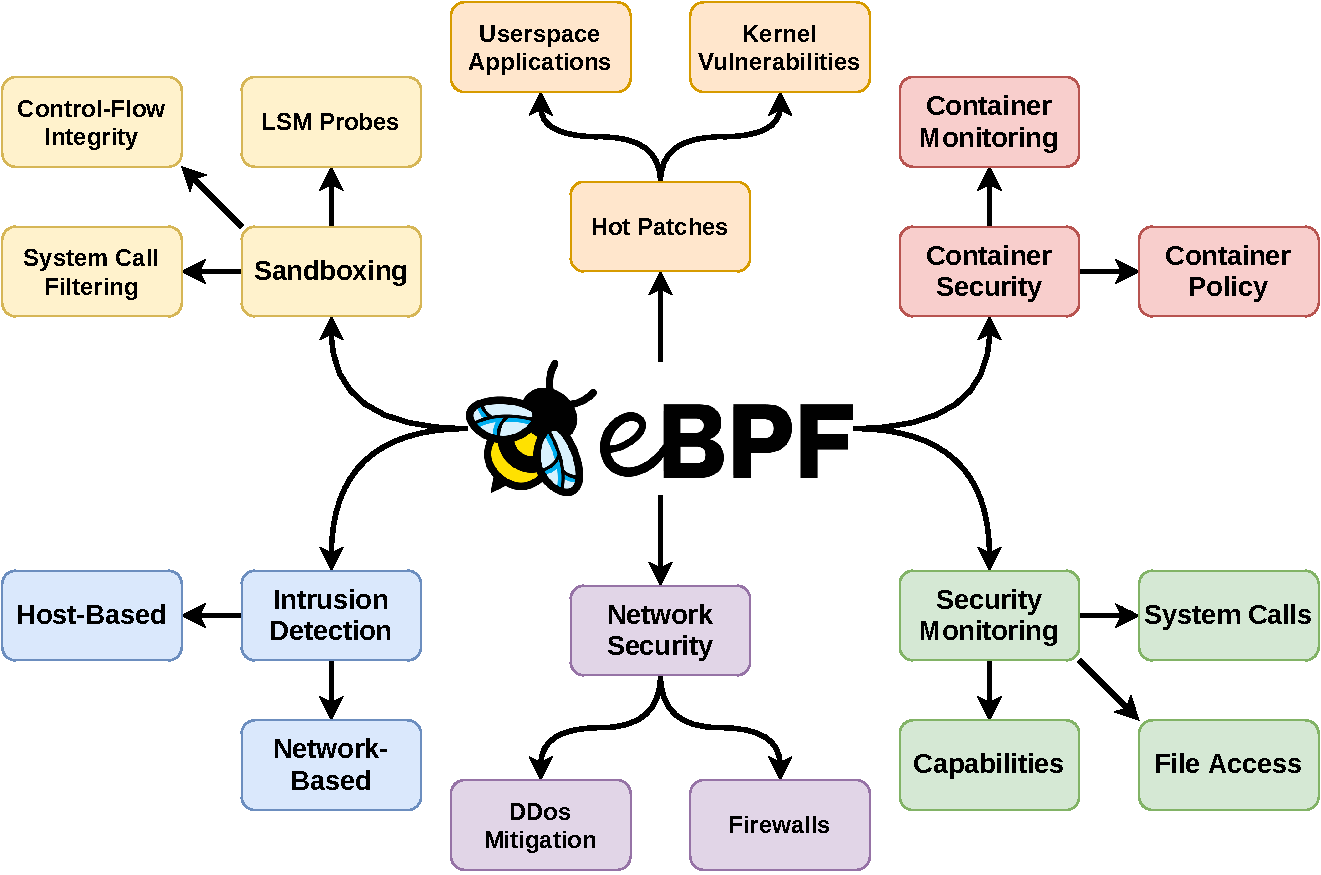
\includegraphics[height=0.8\textheight]{figs/ebpf-security.pdf}
\end{center}
\end{frame}

\begin{frame}[c]{New Directions}
Userspace LSM (Self-Confinement)
\begin{itemize}
    \item Attach \texttt{uprobes} to a shared library
    \item Userspace applications make calls to the library to declare privileges
    \item \texttt{uprobes} update a policy map in kernelspace
\end{itemize}
\vfill
Dynamic Capabilities
\begin{itemize}
    \item Users define custom capabilities
    \item Enforced in kernelspace with dynamic LSM probes
    \item E.g.~\texttt{CAP\_ACCESS\_PHOTOS} to grant access to \texttt{$\sim$/pictures}
\end{itemize}
\end{frame}

\begin{frame}[c]{New Directions}
Hot Patches (Userspace)
\begin{itemize}
    \item Patch vulnerabilities before security updates are available
    \item \texttt{uprobes} to hook into functions
    \item \texttt{bpf\_probe\_write\_user()} to replace userspace memory
\end{itemize}
\vfill
Hot Patches (Kernel)
\begin{itemize}
    \item Replace vulnerable kernel functions with BPF programs
    \item Alter/drop malicious packets before they reach the networking stack
    \item E.g.~patch packet-of-death vulnerability with an XDP program
\end{itemize}
\end{frame}

\section{Conclusion}

\begin{frame}[c]{bpfbox Future Work}
\begin{itemize}
    \item TODO
\end{itemize}
\end{frame}

\begin{frame}[c]{Acknowledgements}
Special thanks to:
\begin{itemize}
    \item \textbf{Alexei Starovoitov} and \textbf{Daniel Borkmann} (creators of eBPF)
    \item \textbf{K.P.~Singh} (creator of KRSI)
    \item Fellow \textbf{bcc contributors} (an awesome eBPF framework)
    \item Anonymous \textbf{CCSW'2020 reviewers} (valuable feedback)
\end{itemize}
\vfill
This work was supported by NSERC through a Discovery Grant.
\end{frame}

\begin{frame}[c]{Contributions}
\begin{itemize}
    \item First \textbf{policy enforcement engine} written in \textbf{eBPF}
    \vfill
    \item Integration of \textbf{userspace} and \textbf{kernelspace} state with \textbf{LSM layer enforcement}
    \vfill
    \item A simple policy language for \textbf{ad hoc process confinement}
    \begin{itemize}
        \item But with optional complexity for \textbf{fine-grained protection}
    \end{itemize}
\end{itemize}
\begin{center}
    
\includegraphics[height=0.4\textheight]{figs/bpfbox-qrcode.eps}\\
    \href{https://github.com/willfindlay/bpfbox}{\ttfamily github.com/willfindlay/bpfbox}\\
    Check out the project on GitHub!
\end{center}
\end{frame}

\end{document}

% vim:syn=tex
